\documentclass[10pt]{beamer}
\usetheme[
%%% options passed to the outer theme
%    hidetitle,           % hide the (short) title in the sidebar
%    hideauthor,          % hide the (short) author in the sidebar
%    hideinstitute,       % hide the (short) institute in the bottom of the sidebar
%    shownavsym,          % show the navigation symbols
%    width=2cm,           % width of the sidebar (default is 2 cm)
%    hideothersubsections,% hide all subsections but the subsections in the current section
%    hideallsubsections,  % hide all subsections
    left               % right of left position of sidebar (default is right)
%%% options passed to the color theme
%    lightheaderbg,       % use a light header background
  ]{AAUsidebar}

% If you want to change the colors of the various elements in the theme, edit and uncomment the following lines
% Change the bar and sidebar colors:
%\setbeamercolor{AAUsidebar}{fg=red!20,bg=red}
%\setbeamercolor{sidebar}{bg=red!20}
% Change the color of the structural elements:
%\setbeamercolor{structure}{fg=red}
% Change the frame title text color:
%\setbeamercolor{frametitle}{fg=blue}
% Change the normal text color background:
%\setbeamercolor{normal text}{bg=gray!10}
% ... and you can of course change a lot more - see the beamer user manual.


\usepackage[utf8]{inputenc}
\usepackage[english]{babel}
\usepackage[T1]{fontenc}
% Or whatever. Note that the encoding and the font should match. If T1
% does not look nice, try deleting the line with the fontenc.
\usepackage{helvet}

%Custom packages
\usepackage{graphicx}
\graphicspath{{graphics/}}

% colored hyperlinks
\newcommand{\chref}[2]{%
  \href{#1}{{\usebeamercolor[bg]{AAUsidebar}#2}}%
}

\title[CHINESE WALL]% optional, use only with long paper titles
{THE CHINESE WALL SECURITY POLICY}

\subtitle{Dr. David F.C. Brewer and Dr. Michael J. Nash, 1989}  % could also be a conference name

\date{November 06, 2015}

\author[Mikael Elki\ae r Christensen] % optional, use only with lots of authors
{
  Mikael Elki\ae r Christensen\\
  \href{mailto:michri11@student.aau.dk}{{\tt michri11@student.aau.dk}}
}
% - Give the names in the same order as they appear in the paper.
% - Use the \inst{?} command only if the authors have different
%   affiliation. See the beamer manual for an example

\institute[
%  {\includegraphics[scale=0.2]{aau_segl}}\\ %insert a company, department or university logo
  Department of Computer Science\\
  Aalborg University\\
  Denmark
] % optional - is placed in the bottom of the sidebar on every slide
{% is placed on the title page
  Department of Computer Science\\
  Aalborg University\\
  Denmark
  
  %there must be an empty line above this line - otherwise some unwanted space is added between the university and the country (I do not know why;( )
}


% specify a logo on the titlepage (you can specify additional logos an include them in 
% institute command below
\pgfdeclareimage[height=1.5cm]{titlepagelogo}{AAUgraphics/aau_logo_new} % placed on the title page
%\pgfdeclareimage[height=1.5cm]{titlepagelogo2}{graphics/aau_logo_new} % placed on the title page
\titlegraphic{% is placed on the bottom of the title page
  \pgfuseimage{titlepagelogo}
%  \hspace{1cm}\pgfuseimage{titlepagelogo2}\textsl{}
}


\begin{document}
% the titlepage
{\aauwavesbg%
\begin{frame}[plain,noframenumbering] % the plain option removes the sidebar and header from the title page
  \titlepage
\end{frame}}
%%%%%%%%%%%%%%%%

\section{Introduction}

\begin{frame}{Who is the enemy?}{}
	\begin{columns}
		\begin{column}{.45\textwidth}
			\includegraphics[width=\textwidth]<2->{graphics/computerninja}
		\end{column}
		\begin{column}{.45\textwidth}
			\includegraphics[width=\textwidth]<3>{graphics/gordongekko}
		\end{column}
	\end{columns}
\end{frame}

\subsection{Background}
\begin{frame}{Background}{}
	\begin{itemize}
		\item Coined in 1929 following the Wall Street crash
		\item Chinese Wall policies are already in use
		\begin{itemize}
			\item Not necessarily digital
			\item Can have authority of law
		\end{itemize}
		\item Other terms, as some find the original offensive
		\begin{itemize}
			\item "Screen", "firewall", "cone of silence", and "ethical wall"
		\end{itemize}
	\end{itemize}
\end{frame}

\subsection{Relevance}
\begin{frame}{Relevance}{}
	\begin{itemize}
		\item Before 1989, most security policies were military
		\begin{itemize}
			\item E.g. Bell-LaPadula (more about this later)
		\end{itemize}
		\item Need of something that holds up in court
		\item Relevant anywhere conflicts of interest can exist
	\end{itemize}
\end{frame}

%%%%%%%%%%%%%%%%

\section{Bell-LaPadula}

\begin{frame}{Bell-LaPadula}{}
	\begin{itemize}
		\item Proposed by Bell and LaPadula in 1973
		\item Security policy model
		\item Designed for military use
	\end{itemize}
\end{frame}

\subsection{Terminology}
\begin{frame}
	\frametitle{Terminology}
	
	\begin{itemize}
		\item \textbf{Security Label}
		\item \textbf{Object} -- Data or program
			\begin{itemize}
				\item \textbf{Classification} -- Minimum security level
				\item \textbf{Category} -- Security group(s)
			\end{itemize}
		\item \textbf{Subject} -- Person or program
			\begin{itemize}
				\item \textbf{Clearance} -- Maximum security level
				\item \textbf{Need-to-know} -- Security group(s)
			\end{itemize}
	\end{itemize}
\end{frame}

\subsection{Access rules}
\begin{frame}
	\frametitle{Access rules}
	
	\begin{description}
		\item[Simple security:] access is granted only if the subject's clearance is \textit{greater} than the object's classification and the subject's need-to-know \textit{includes} the object's category(ies)
		\item[*-property:] write access is granted only if the output object's classification is \textit{greater} than the classification of all input objects, and its category \textit{includes} the category(ies) of all input objects.
	\end{description}
\end{frame}

\subsection{Example}
\begin{frame}
	\frametitle{Example}
	
	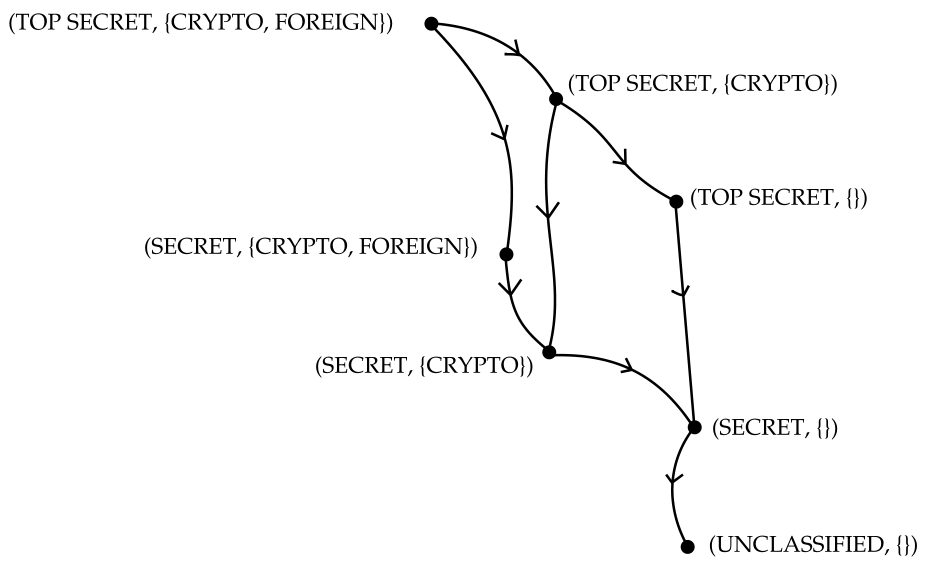
\includegraphics[width=\textwidth]{graphics/blp_lattice}
\end{frame}

\begin{frame}
	\frametitle{Example (2)}
	
	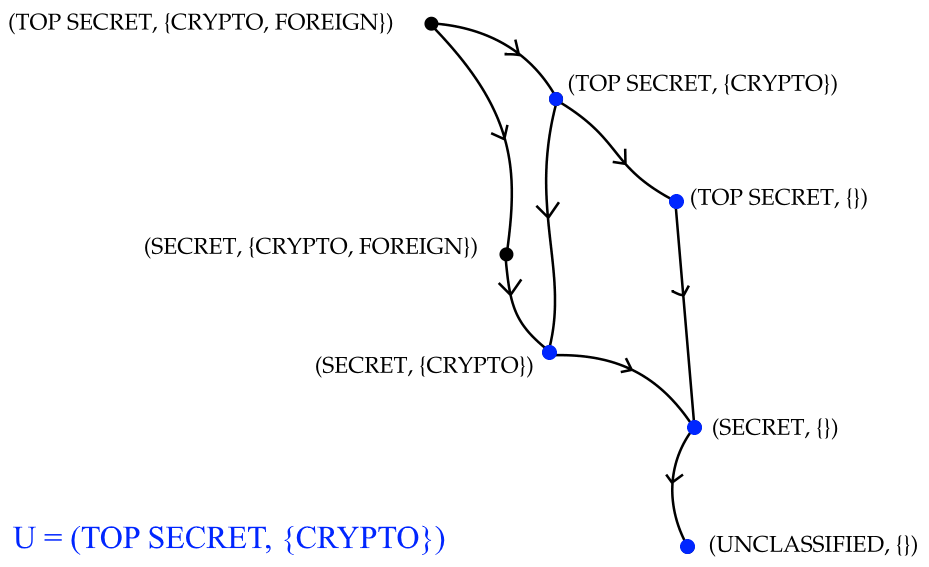
\includegraphics[width=\textwidth]{graphics/blp_lattice_2}
\end{frame}


{\aauwavesbg
\begin{frame}[plain,noframenumbering]
	\finalpage{Questions?}
\end{frame}}
%%%%%%%%%%%%%%%%

\end{document}
